\chapter{Implementierung}
\label{cha:implementierung}

% Abschnitt: Implementierungsdetails
\section{Implementierungsdetails}
\label{sec:implementierung:implementierungsdetails}

In diesem Abschnitt möchten wir ein wenig genauer auf unsere Quartett App und ihre Funktionen eingehen. Dies machen wir ausgehend vom Hauptmenü aus, welches in Abbildung \ref{figure:implementierungmenue} zu sehen ist. Für das Hauptmenü wir, wie auch für die gesamte App, haben wir ein ansprechendes Farbklima gewählt.

\begin{figure}[htp]
	\centering
  	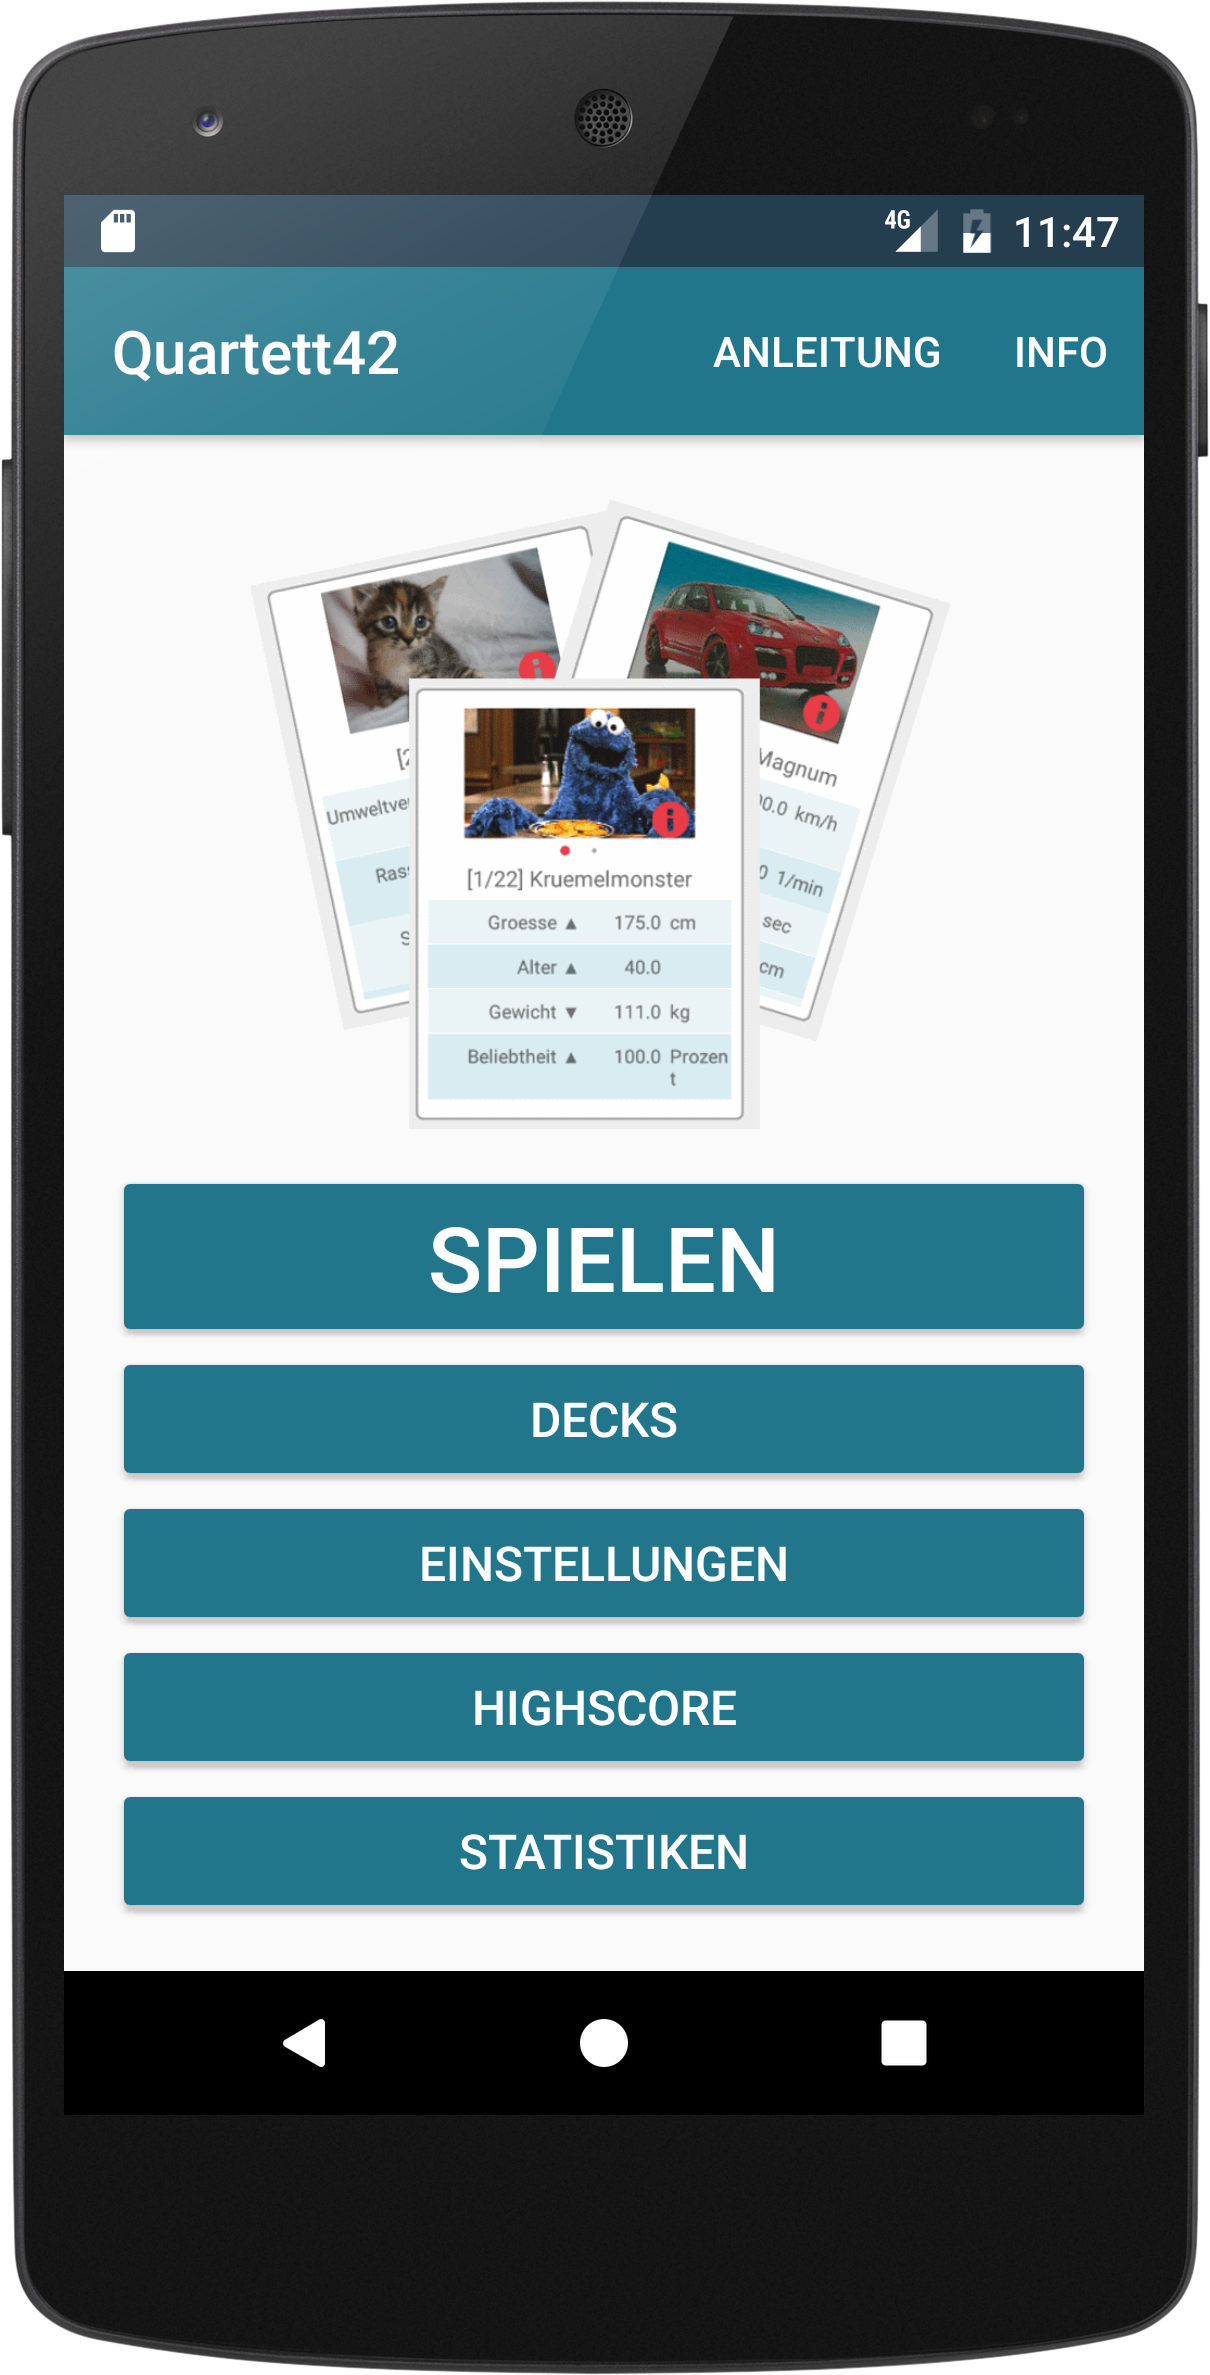
\includegraphics[width=0.3\textwidth]{img/screenshots/device_main_screen.png}
	\caption{Das Hauptmenü der Quartett42 App}
	\label{figure:implementierungmenue}
\end{figure}

Durch den Menüpunkt "SPIELEN" landet der Spieler auf einem Bildschirm, in welchem er ein Deck wählen kann und bei Bedarf die Einstellungen anpassen kann, wie in Abbildung \ref{figure:implementierungeinstellungen} zu sehen ist. Diese sind frei wählbar und alle Kombinationen sind möglich. Die Einstellungen werden lokal auf dem Smartphone gespeichert und können beim nächstmaligen Starten direkt übernommen werden, ohne sie jedes mal neu zu ändern. Das ermöglicht einen schnellen Start ins Spiel.

\begin{figure}[htp]
	\centering
  	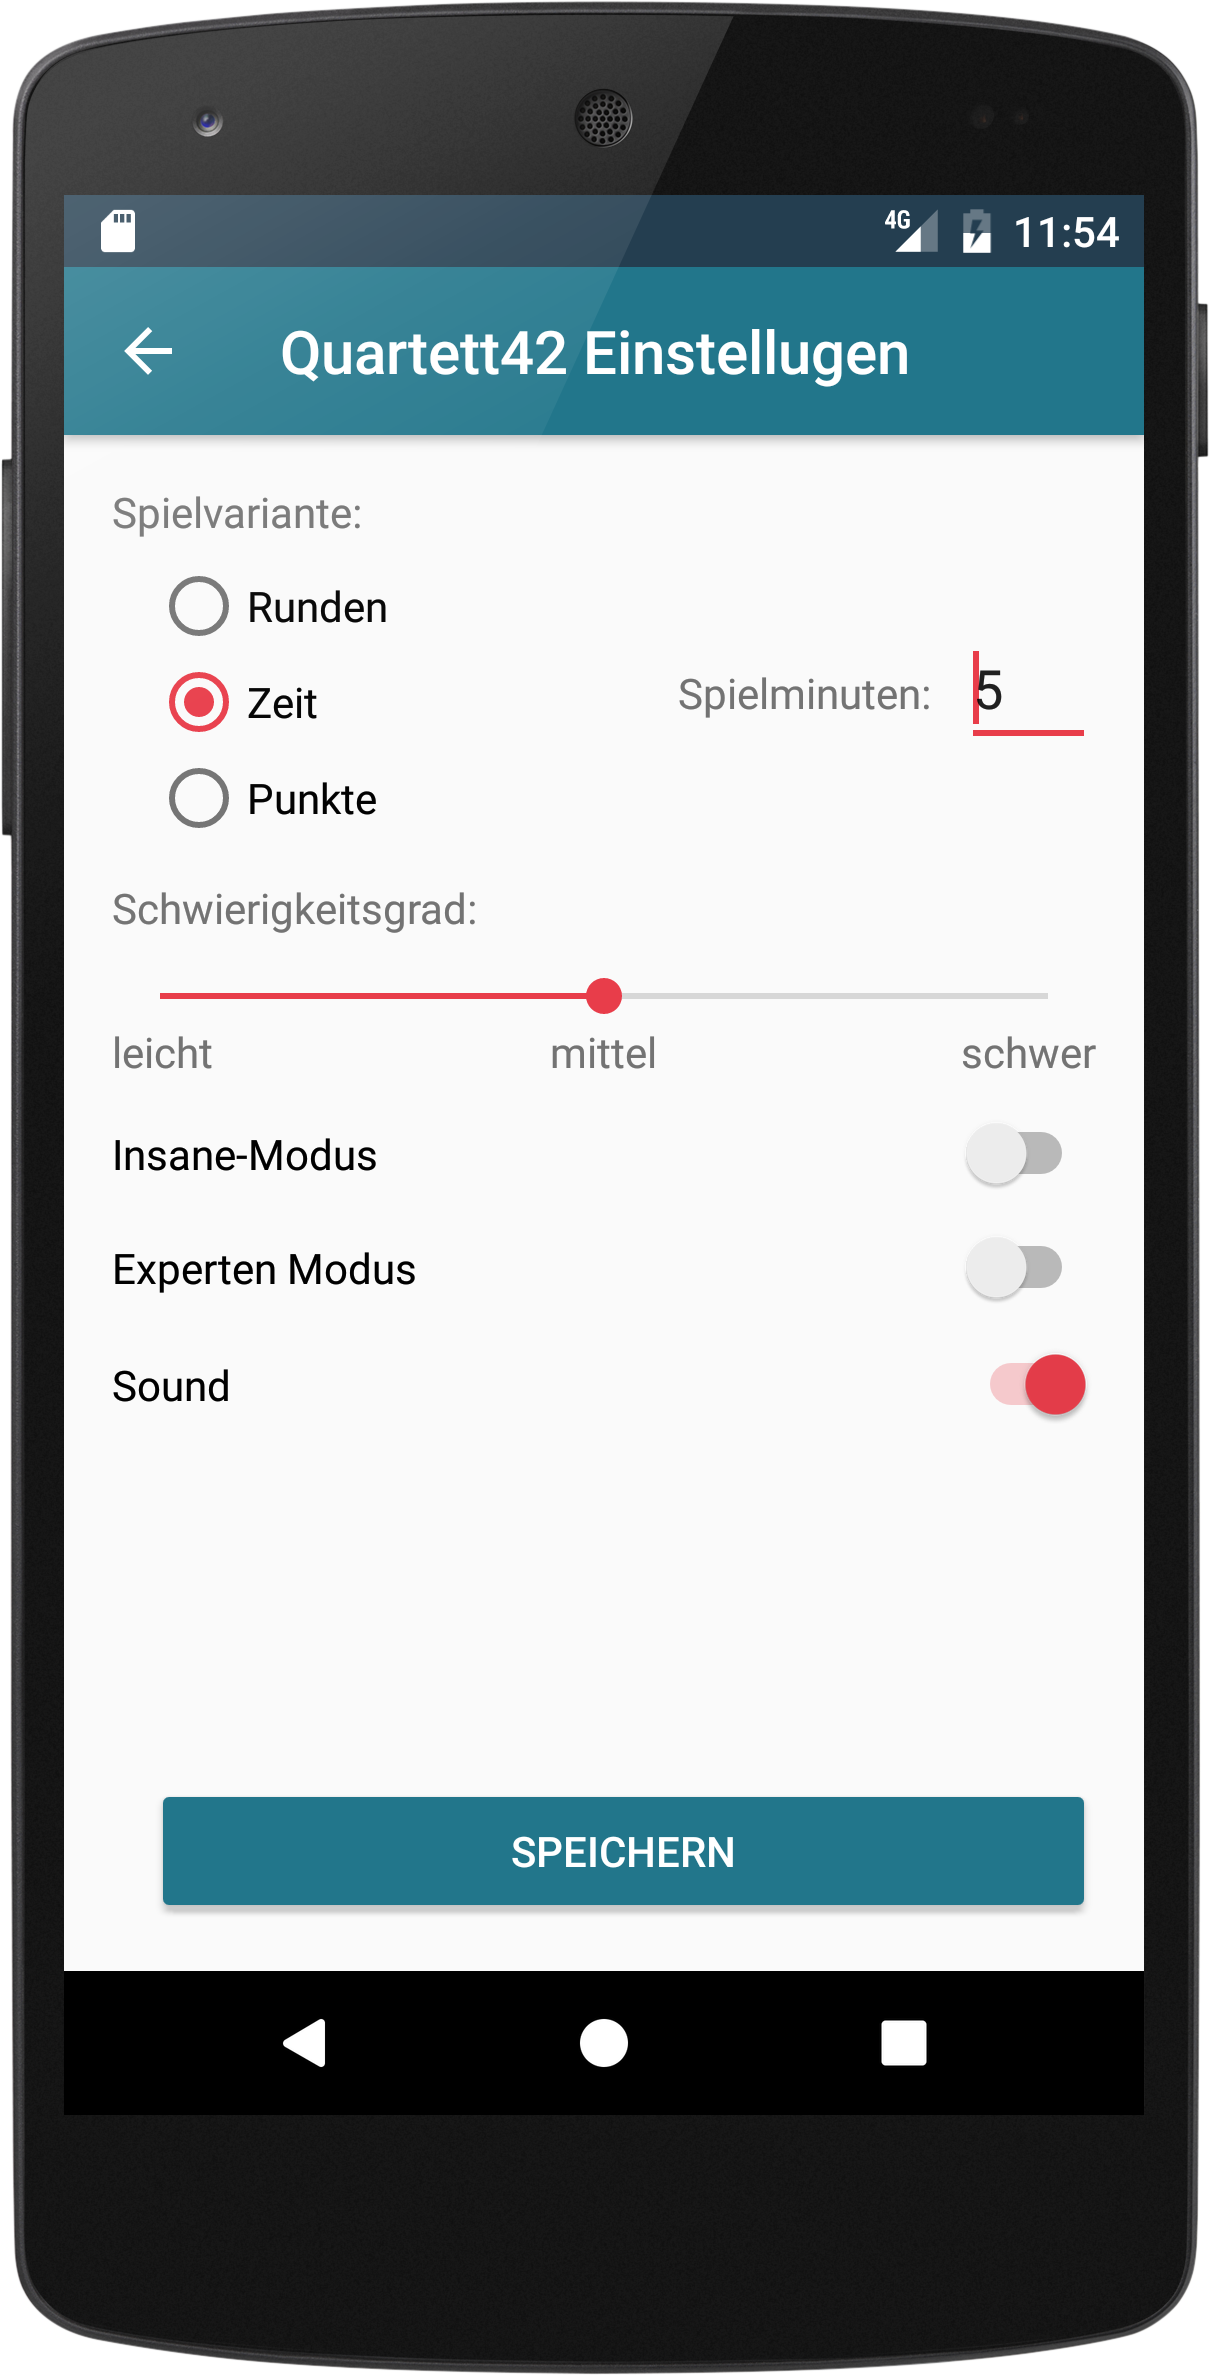
\includegraphics[width=0.3\textwidth]{img/screenshots/device_settings.png}
	\caption{Das Einstellungsmenü der Quartett42 App}
	\label{figure:implementierungeinstellungen}
\end{figure}

Nun ist das eigentliche Spiel gestartet. Der Spieler sieht jeweils nur seine erste oberste Karte, wie in Abbildung \ref{figure:implementierungspiel1} abgebildet ist. Für jedes Attribut wird neben dem Wert (beziehungsweise einem Fragezeichen im "Expertenmodus") auch die jeweilige Einheit und die Siegesvariante (höher oder niedriger gewinnt) angegeben. Zwischen den Bildern einer Karte kann durch Swipe-Gesten gewechselt werden und zu jedem Bild kann, falls vorhanden, die passende Information durch drücken auf den Info-Buttonn angezeigt werden. Wenn der Spieler am Zug ist, sind seine Attribute aktiv und er kann ein Attribut für den Vergleich auswählen. Für seinen Zug hat der Spieler unbegrenzt Zeit, außer im Zeitmodus, in welchem die Zeit für einen Zug auf 30 Sekunden beschränkt ist, damit der Spieler sich nicht auf seinen bisherigen Erfolgen ausruhen kann. Die Zeit für seinen Zug wird ihm angezeigt und zudem werden die letzten 10 Sekunden durch ein akustisches Signal verdeutlicht, sofern in den Einstellungen die Sounds aktiviert sind. In allen Spielvarianten wird dem Spieler während des Spiels der aktuelle Zwischenstand (durch Punkte oder Karten) und die verbliebende Spielzeit(verbleibende Karten/Punkte/Zeit) angezeigt.

\begin{figure}[htp]
	\centering
  	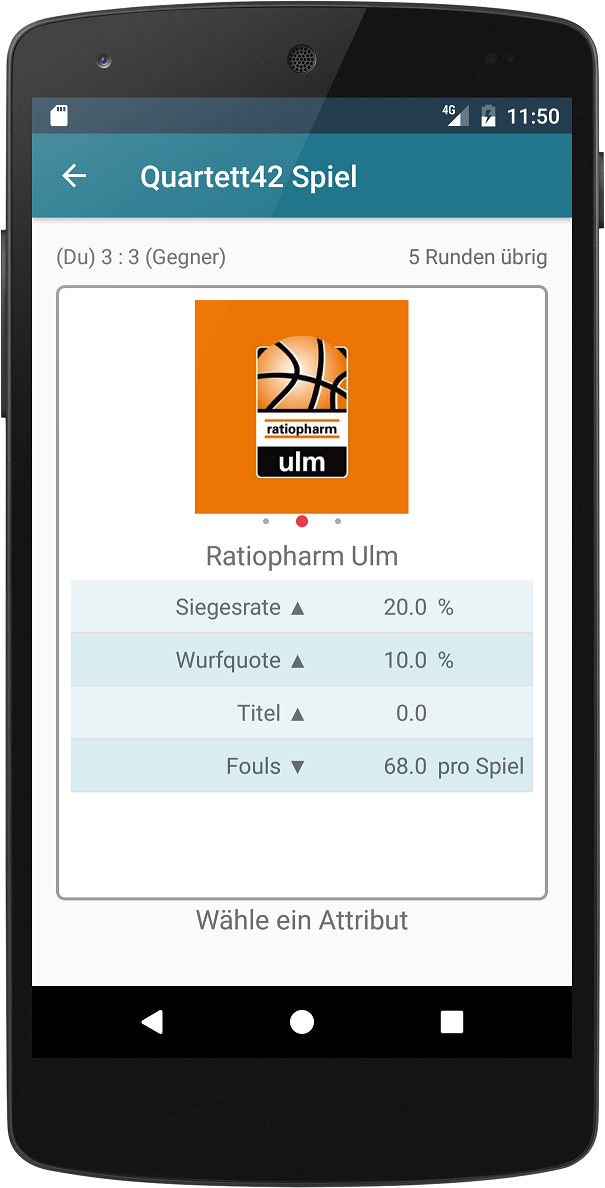
\includegraphics[width=0.3\textwidth]{img/screenshots/device_select_attr.png}
	\caption{Kartenansicht während eines laufenden Spiels}
	\label{figure:implementierungspiel1}
\end{figure}

Ist der Gegner am Zug, sieht die Kartenansicht des Spielers gleich aus, aber seine Attribute sind inaktiv und nicht auswählbar. Nun muss der Spieler eine gewisse Zeit warten, bis der Computer sein Attribut für den Vergleich ausgewählt hat. Diese Zeit kann er nutzen, um seine Karte zu betrachten. Im Schwierigkeitsgrad "leicht" wählt der Computer ein zufälliges Attribut für den Vergleich aus. Im Schwierigkeidsgrad "mittel" wählt er unter einer zufälligen Menge an Attributen, welche ungefähr die Mächtigkeit der Hälfte aller Attribute hat, den besten Wert aus. Im Schwierigkeitsgrad "schwer" wählt der Computer unter allen Attributen zu einer gewissen Wahrscheinlichkeit den besten Wert aus. Diese Schwierigkeitsgrade sorgen dafür, dass der Spieler zwar einen Anstieg der Schwierigkeit des Computers spürt, jedoch immer eine Chance zu gewinnen hat. Zudem bliebt durch die Zufallswerte der Zug des Computergegners unvorhersehbar.

Nach jedem gespielten Zug sieht der Spieler den Vergleichsbildschirm mit seiner Karte und der Karte seines Gegners, wie in Abbildung \ref{figure:implementierungspiel2}  dargestellt. Dort kann wieder bei beiden Karten zwischen den Bildern durch Swipe-Bewegungen gewechselt werden und die jeweiligen Informationen durch Drücken des Info-Buttons angesehen werden. Der gewählte Wert beider Spieler wird angezeigt und der Gewinner hervorgehoben. Der Gewinner bekommt beide Karten, bei einem Unentschieden behält jeder Spieler seine Karte. Zudem wird der Punktestand aktualisiert. Im Kartenmodus und im Zeitmodus ist jede Karte genau ein Punkt wert. Im Punktemodus berechnen sich die Punkte für den Gewinner durch den prozentualen Unterschied beider Werte. So kann der Spieler mit ein und dem selben Attribut einer Karte unterschiedlich viele Punkte machen, je nachdem welche Karte der Gegner gerade besitzt. Außerdem ist es dadurch möglich, dss ein Spieler mit weniger Karten als der Gegner gewinnt, weil er durch geschickte Spielzüge mehr Punkte gesammelt hat.

\begin{figure}[htp]
	\centering
  	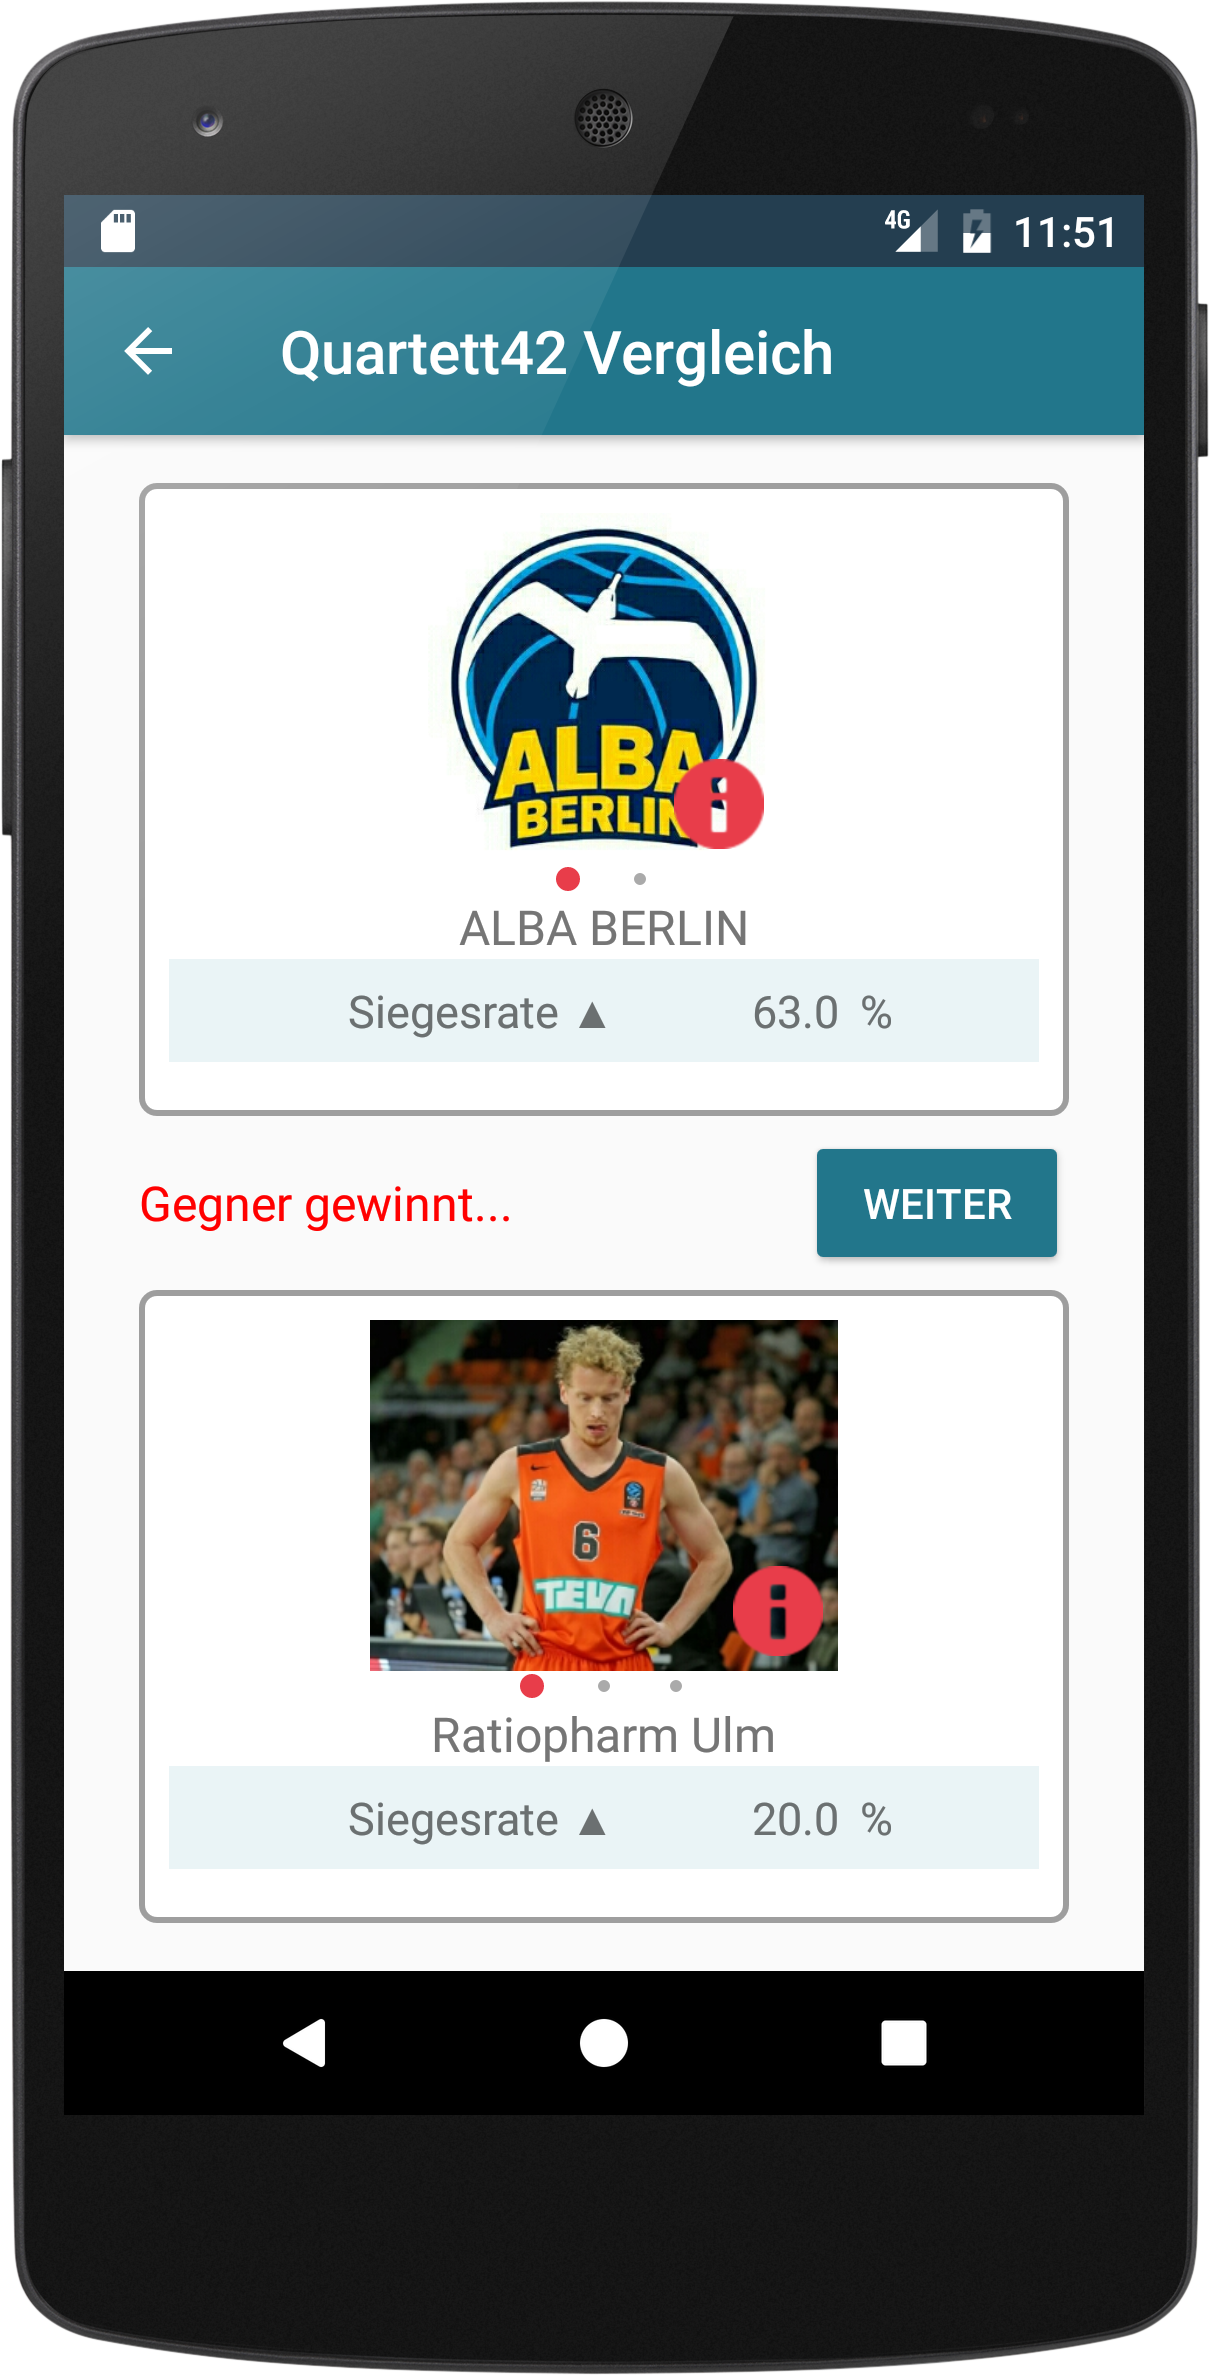
\includegraphics[width=0.3\textwidth]{img/screenshots/device_comparison.png}
	\caption{Kartenvergleich nach jedem Zug}
	\label{figure:implementierungspiel2}
\end{figure}

Der Spieler hat jederzeit die Möglichkeit, das laufende Spiel zu unterbrechen. Dazu wird ein Spiel automatisch zwischengespeichert, wenn der Spieler das laufende Spiel oder die App verlässt. Dieses kann der Spieler zu einem späteren Zeitpunkt fortsetzen. Wenn er ein neues Spiel beginnen möchte wird er gefragt, ob er lieber das alte Spiel fortsetzen will oder ein neues beginnen und das alte überschreiben möchte.

Steht ein Gewinner fest, wird der Spielend-Bildschirm angezeigt. Auf diesem steht der Gewinner, der Endstand und die gesammelten Punkte des Gewinners. Ist der Spieler der Gewinner, wird anhand dieser Punkte entschieden, ob der Spieler es in die Rangliste geschafft hat, und falls ja, auf welche Position. Die Punkte berechnen sich durch eine Kombination aus den gesammelten Punkten im Spiel, dem Schwierigkeitsgrad des Spiels, dem Spielmodus (normal, Insanemodus oder Expertenmodus) und der Anzahl der eingestellten Runden/Zeit/Punkte. Dadurch bleibt die Rangliste immer fair und kann nicht durch vereinfachte Einstellungen oder eine erhöhte Anzahl an Spielrunden beeinflusst werden. Der Spieler kann sich hier direkt mit seinem Namen in die Rangliste eintragen, wobei der jeweils letzte Name gespeichert wird. Außerdem kann er von diesem Bildschirm direkt die Ranglisten (Abbildung \ref{figure:implementierungrangliste}) einsehen oder eine Revanche starten, welche ein Spiel mit dem gleichen Deck und den gleichen Einstellungen startet.

\begin{figure}[htp]
	\centering
  	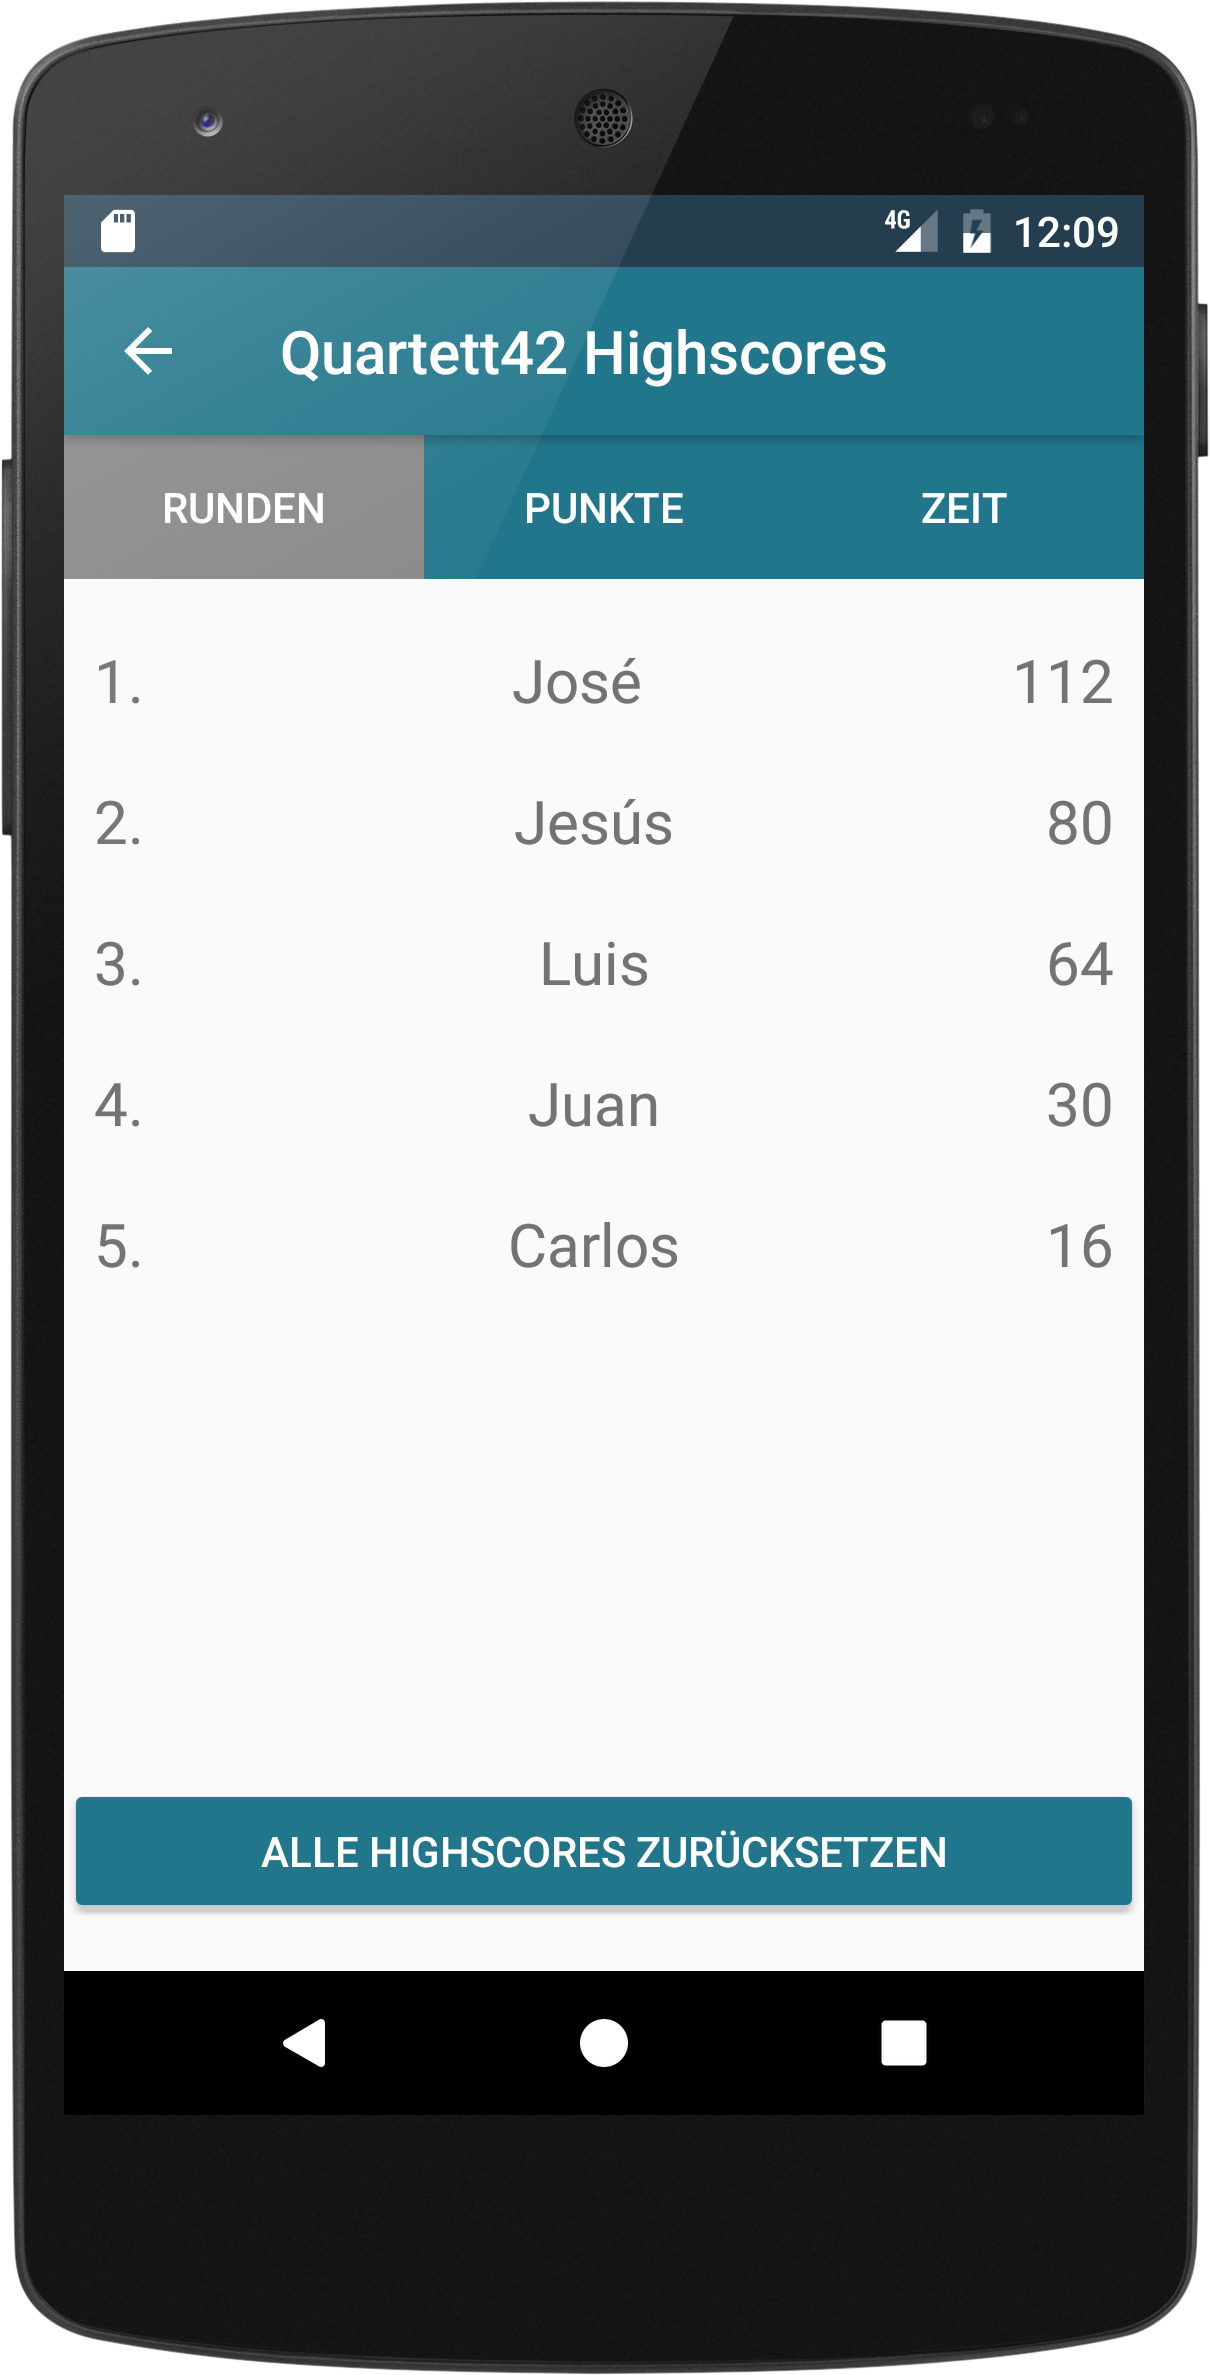
\includegraphics[width=0.3\textwidth]{img/screenshots/device_high_scores.png}
	\caption{Die Rangliste der Quartett42 App}
	\label{figure:implementierungrangliste}
\end{figure}

Neben dem Spiel ansich befinden sich die meisten Implementierungsdetails unserer Anwendung im Menüpunkt "GALERIE". Dort hat der Spieler eine Übersicht aller Decks, die auf dem Smartphone vorhanden sind. Dieses Menü wurde durch ein Grid-Layout-Adapter erstellt und findet sich an vielen Stellen in unserer App wieder. Es erlaubt neben einer einfachen und immer gleich großen und gleich formartierten Darstellung der Bilder auch ein einfaches Scrollen und Anzeigen von Deckinformationen durch drücken auf den Info-Button. Ein Bild davon gibt es in Abbildung \ref{figure:implementierunggalerie} Im Menü kann der Spieler die Karten eines Decks angucken, was ungefähr ähnlich ausieht wie die Kartenansicht während eines Spiels in Abbildung \ref{figure:implementierungspiel1}. Zudem kann er hier die Namen der Decks umbenennen, die einzelnen Werte und Bilder mit dazugehörigen Beschreibungen einzelner Karten der Decks ändern sowie neue Karten zu Decks hinzufügen oder Karten löschen. Außerdem kann ein Deck auch gelöscht werden oder über den Deckcreator ein völlig neues Deck mit neuen Attributen erstellt werden. Neue Decks können dann auf den Deckstore hochgeladen werden, sodass es für andere Nutzer zur Verfügung steht. Über diesen können wiederum auch neue Decks von anderen Nutzern auf das Smartphone herunter geladen werden. Auf diese zuletzt genannten Funktionen werden wir in den Besonderheiten genauer eingehen. 

\begin{figure}[htp]
	\centering
  	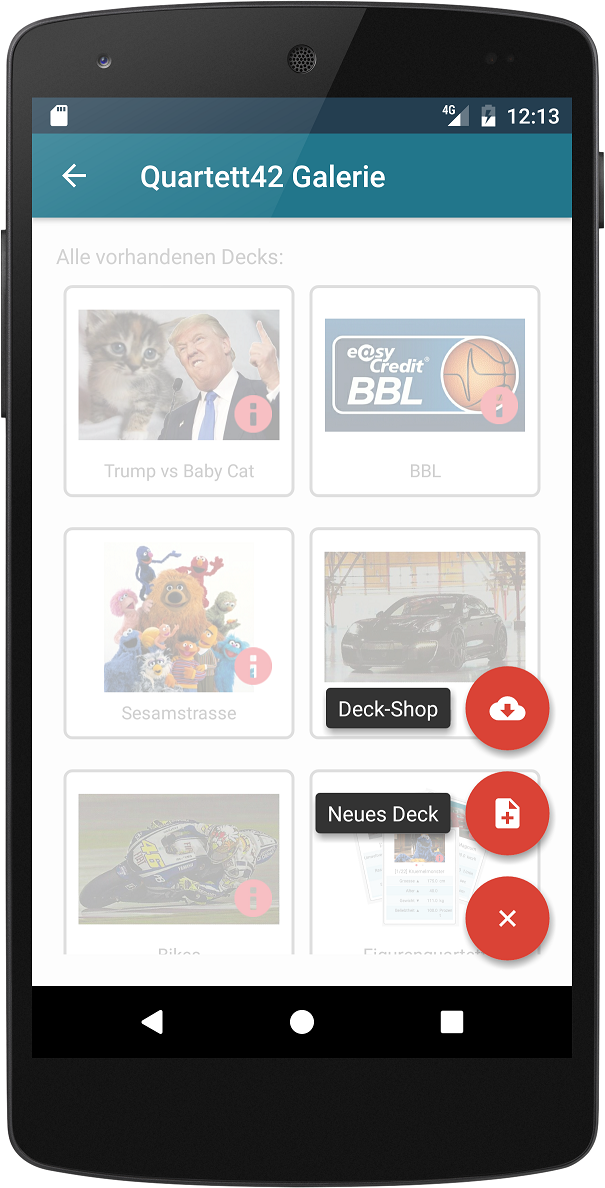
\includegraphics[width=0.3\textwidth]{img/screenshots/device_gallery.png}
	\caption{Die Galerie mit allen heruntergeladenen Decks und ein Teil ihrer Funktionen}
	\label{figure:implementierunggalerie}
\end{figure}

Neben der Rangliste gibt es auch noch einige Statistiken in unserer App, wie zum Beispiel die Anzahl der gepsielten Spiele und die dabei gewonnen und verlorenen Spiele für die verschiedenen Spielmodi. Diese werden mit Hilfe der Bibliothek MPAndroidCharts als Piechart dargestellt und werden nach jedem bis zum Ende durchgespielten Spiel aktualisiert. Ein Bild davon gibt es in Abbildung \ref{figure:implementierungstatistiken}.

\begin{figure}[htp]
	\centering
  	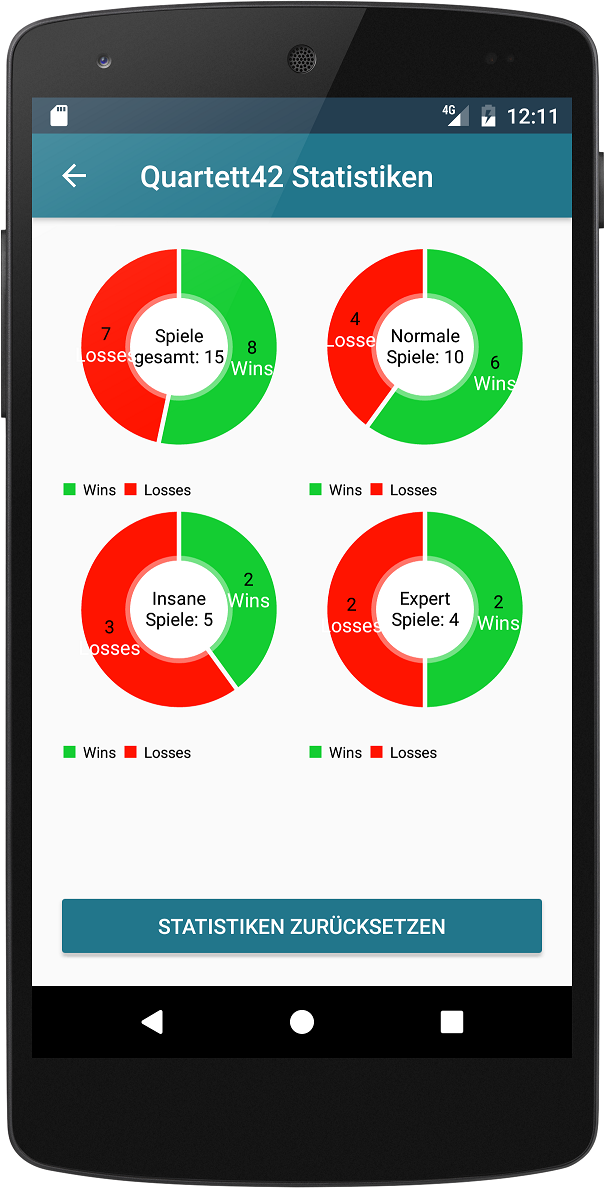
\includegraphics[width=0.3\textwidth]{img/screenshots/device_statistics.png}
	\caption{Die Ansicht der Statistiken}
	\label{figure:implementierungstatistiken}
\end{figure}

% Abschnitt: Architektur
\section{Architektur}
\label{sec:implementierung:architektur}

TODO

- ein paar Einleitungssätze
- Datenmodell aus Präsentation kopieren und erlüutern, was besonders ist (auf Speicherung mit JSON eingehen)
- Klassen-/Activity-Modell aus Präsentation kopieren
- vielleicht ein paar Sätze zu allgemeinem Vorgehen und Aufteilung??

% Abschnitt: Besonderheiten 
\section{Besonderheiten}
\label{sec:implementierung:besonderheiten }

Im Vergleich zu anderen Quartett Apps gibt es bei unserer Quartett42 App, neben den verschiedenen Spielmodi und Decks, besonders zwei Funktionen, die so bisher noch nicht verfügbar waren. Diese sind zum einen unser Deckcreator und -editor und zum anderen der Deck Down- und Upload.	

\subsection{Deckcreator und -editor}
\label{sec:implementierung:besonderheiten:deckcreator }

\begin{figure}[htp]
	\centering
  	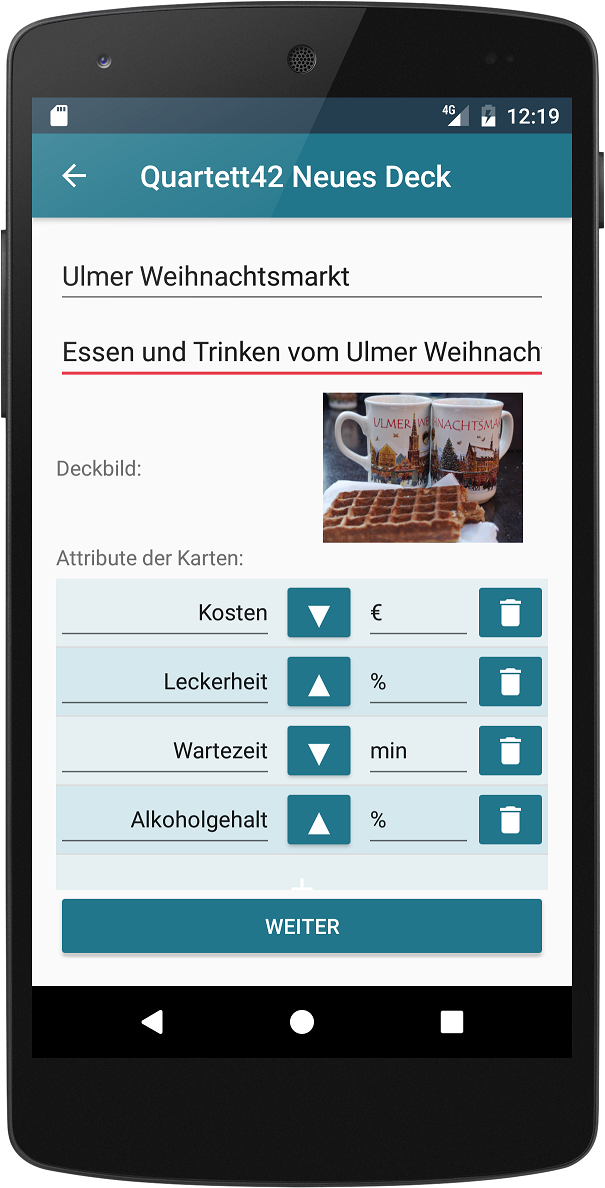
\includegraphics[width=0.3\textwidth]{img/screenshots/device_new_deck.png}
	\caption{Erster Schritt im Deckcreator}
	\label{figure:implementierungdeckcreator}
\end{figure}

Der Deckcreator erlaubt das Erstellen neuer Decks oder das Bearbeiten vorhandener Decks. Dadurch kann jeder Spieler ein komplett neues eigenes Deck nach seinen Wünschen erstellen. Über die Galerie gelangt der Spieler in den Deckcreator. Dort muss er erst einmal allgemeine Angaben zu seinem gewünschten Deck angeben, wie in Abbildung \ref{figure:implementierungdeckcreator} dargestellt. Dort mus ein Namen für das Deck eingegeben werden, wobei der Creator ein Deck nur erstellt, wenn dieser Name nicht bereits vergeben ist. Beschreibung und Bild sind optional, wobei bei keinem angegebenem Bild ein Standardbild verwendet wird. Das Bild kann entweder aus der Fotogalerie des Smartphones gewählt werden oder direkt aufgenommen werden, wobei es in beiden Fällen direkt auf eine akzeptable Größe verkleinert wird. Zudem müssen eine beliebige Anzahl an Attributen festgelegt werden, und für jede Attribut, wann es gewinnt, und welche Einheit es hat. Hier müssen verschiedene Überprüfungen statt finden. So darf kein Attribut zwei mal verwendet werden und es dürfen nirgends unerlaubte Zeichen oder leere Eingaben vorkommen. Sind alle Eingaben korrekt, wird das Deck zwischen gespeichert und der Nutzer zum zweiten Schritt weiter geleitet.

\begin{figure}[htp]
	\centering
  	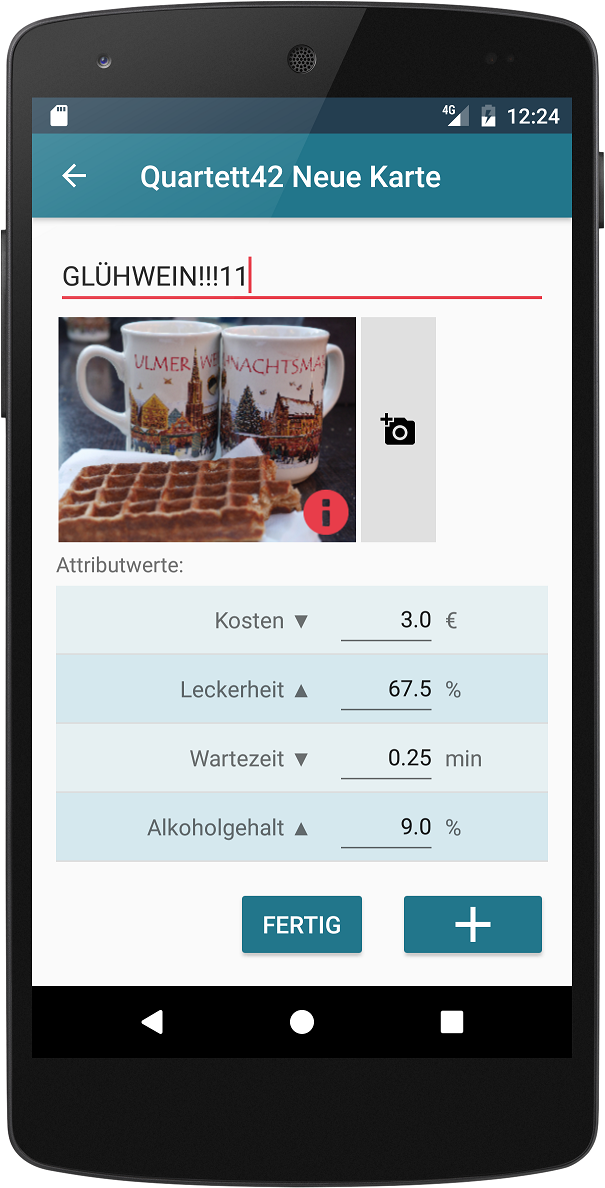
\includegraphics[width=0.3\textwidth]{img/screenshots/device_new_card.png}
	\caption{Zweiter Schritt im Deckcreator}
	\label{figure:implementierungdeckeditor}
\end{figure}

Im zweiten Schritt geht es um die Erstellung einzelner Karten und deren Werte. Wenn der Benutzer ein bereits vorhandenes Deck bearbeiten will, gelangt er direkt in diesen Schritt. Ein Bild davon kann man in Abbildung \ref{figure:implementierungdeckeditor} sehen. Für jede Karte muss ein Name eingegeben werden, welcher pro Deck wieder nur einmal vorkommen darf. Zudem kann eine beliebige Anzahl an Bildern wie beim Deckbild und dazu passende Beschreibungen angegeben werden. Für jedes Attribut der Karte muss ein Wert angegeben werden. Auch hierbei muss wieder alles auf gültige Eingaben überprüft werden und es dürfen keine leeren Eingaben vorkommen. Der Spieler kann jederzeit eine neue Karte hinzufügen und eine alte Karte löschen. Zudem kann er zwischen allen Karten hin und her wechseln. Dabei wird das Deck bei jedem Wechsel zwischengespeichert. Damit ein Deck spielbar ist, muss es mindestens zwei Karten besitzen. Ist der Nutzer fertig mit dem Erstellen oder Bearbeiten eines Decks, kann er es speichern und ansehen oder spielen. Zudem besteht die Möglichkeit, den Erstellvorgang zu unterbrechen und zu einer anderen Zeit fortzusetzen.

\subsection{Down- und Upload von Decks}
\label{sec:implementierung:besonderheiten:deckdownload }

Über den Deckstore können neue Decks runter und hoch geladen werden. Das ermöglicht das Teilen von selbst erstellten Decks mit anderen und führt dazu, dass immer wieder neue Decks herunter geladen werden können. Die Speicherung der Decks findet auf einem Server des Institutes für Datenbank und Informationssysteme der Universität Ulm statt. Die Daten Decks werden dabei als JSON-Strings gespeichert. 

Über die Galerie gelangt man in den Deckstore, in welchem dem Spieler alle Decks aus dem Deckstore angezeigt werden, welche er noch nicht selbst auf sein Smartphone herunter geladen hat. Diese erfragt die Anwendung durch einen Http-Request an den Server, welcher eine Liste alle auf dem Server vorhandenen Decks zurück liefert. Zudem wird für jedes Deck noch das Deckbild und die Deckbeschreibung herunter geladen und gecached. Außerdem erhält der Nutzer beim Starten der App eine Notifikation in der Statusleiste, falls neue Decks im Decksotre verfügbar sind. Die Darstellung im Deckstore erfolgt wieder über den Grid-View-Adapter, ähnlich zu Abbildung \ref{figure:implementierunggalerie}. Der Benutzer kann nun ein Deck auswählen, welches er herunterladen möchte. Der Nutzer sieht während dem gesamten Ladevorgang einen Fortschrittsbalken, welcher den Fortschritt in Prozent berechnet und darstellt. Für das Deck wird dann zuerst die allgemeine Deckinformation heruntergeladen sowie eine Liste aller Karten. Dann wird jede einzelne Karte heruntergeladen und für jede Karte alle dazugehörigen Bilder und Werte. Für jede dieser Daten wird ein Http-Request an den Server gesendet, welcher die Daten in Form eines JSON-Strings zurück gibt. Da nicht nur unsere Anwendung sondern mehrere Anwendungen Decks auf den Server hochladen können, welche nicht unbedingt formal korrekt sein können, wird in jedem Schritt überprüft, ob das Deck alle Anforderungen erfüllt. Dazu gehören zum Beispiel eine Mindestanzahl an Karten und Attributen, keine unerlaubten Zeichen und leere Angaben sowie keine falschen Bilddateien. Letzteres wird durch ein Standardbild ersetzt, bei allen anderen Fehlern wird der Download abgebrochen, um unnötige Wartezeiten zu vermeiden. Bilder, die zu groß sind, werden automatisch verkleinert. Nach dem vollständigen Download aller Daten und der Kontrolle wird das Deck zusammen gebaut und in den lokalen Speicher gespeichert. Hierbei wird bevozugt versucht, die Daten auf einem externen Speicher zu speichern, um nicht den internen speicher zu belasten. Eine Grafik, wie der Download funktioniert, sieht man in Abbildung \ref{figure:implementierungdownundupload}.

In der Galerie hat der Benutzer die Möglichkeit, ein Deck direkt auf den Server hochzuladen. Zuerst wird durch eine Anfrage an den Server überprüft, ob das Deck schon im Deckstore vorhanden ist. Ist dies der Fall, kann das selbe Deck nicht erneut hochgeladen werden. Fall nicht, bekommt der Benutzer wieder eine Ladeanzeige mit Fortschrittsbalken zu sehen. Bevor das Deck hochgeladen wird, wird auch dieses zur Sicherheit auf Fehler überprüft, welche aber im Normalfall dank der Fehlerüberprüfung bei der Deckerstellung nicht vorkommen dürfen. Dann wird das Deck in viele einzelne JSON-Strings zerlegt und dem Server über einen Http-Request das Deck mit seinen Informationen bekannt gegeben. Danach wird wie beim Download, jede Karte und mit ihm seine Werte Werte und Bilder als JSON-String über einen extra Http-Request gesendet, wobei die Bilder in einen Base64-String konvertiert und versendet werden. Nach dem vollständigen Upload ist das Deck für alle Benutzer über den Deckstore verfügbar. Eine Grafik, wie der Upload funktioniert, sieht man in Abbildung \ref{figure:implementierungdownundupload}. Sollte der Benutzer keine Internetverbindung, wird sowohl der Download als auch der Upload abgebrochen.
\newpage

%Download- und Upload-Verlauf-Modell
\begin{figure}[htp]
\centering
\begin{minipage}{.45\textwidth}
  \centering
  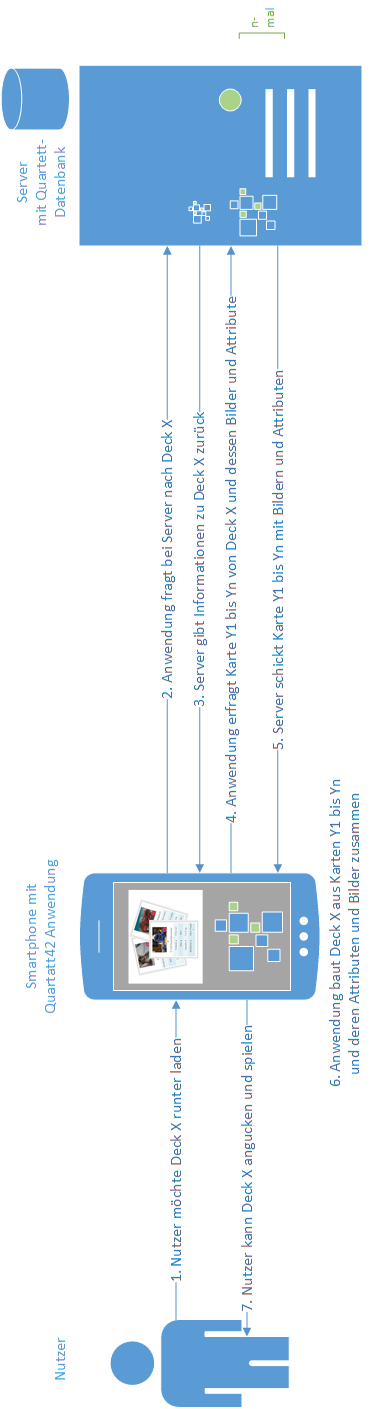
\includegraphics[width=.95\linewidth]{img/modelle/downloadmodell.png}
\end{minipage}%
\begin{minipage}{.45\textwidth}
  \centering
  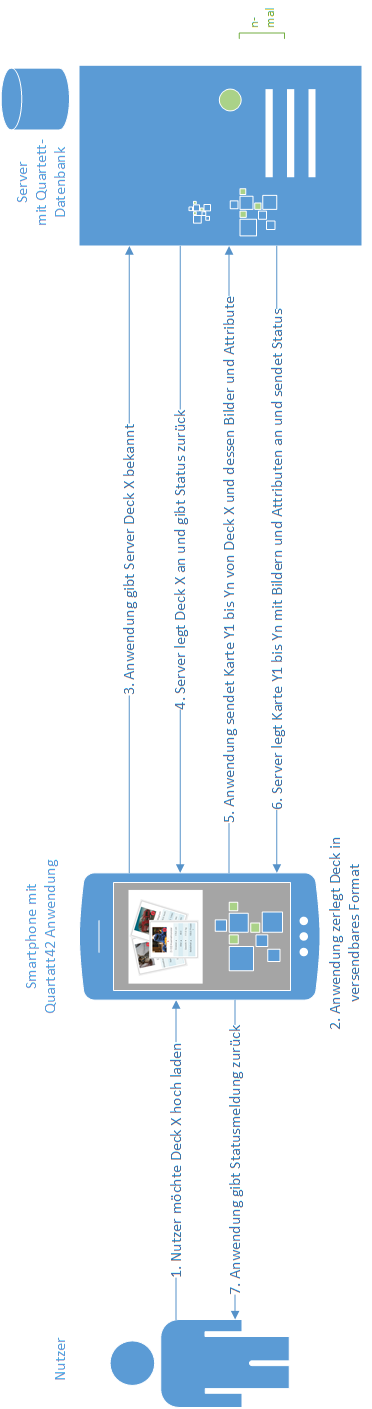
\includegraphics[width=.95\linewidth]{img/modelle/uploadmodell.png}
\end{minipage}%
\caption{Links: Downloadmodell, rechts: Uploadmodell }
\label{figure:implementierungdownundupload}
\end{figure}
\newpage

% Abschnitt: Schwierigkeiten während der Implementierung 
\section{Schwierigkeiten während der Implementierung}
\label{sec:implementierung:schwierigkeiten }	

TODO

Wie in Präsentation